% 2015-05-21 - Emerson Ribeiro de Mello - mello@ifsc.edu.br
% \documentclass[handout,xcolor=pdftex,dvipsnames,table]{beamer}
\documentclass{beamer}

\usepackage[utf8]{inputenc}
\usepackage[T1]{fontenc}
\usepackage[english]{babel}
\usepackage{float}
\usepackage{graphics}



% usando tema personalizado. 
% arquivo beamerthemeIFSC.sty deve estar no mesmo diretório do .tex
\usepackage{beamerthemeIFSC}

\usepackage{amsmath}

\hypersetup{pdfstartview={Fit},pdftitle={\@title},
 	pdfsubject={Introduction to MATLAB},pdfauthor={\@author}
}

%%%%%%%%%%%%%%%%%%%%%%%%%%%%%%%%%%%%%%%%%%%%


\title{Introduction to MATLAB}
\author{Ahmad Asadi}
\date{Spring 2016}
\institute{Amirkabir University of Technology\\
Department of Computer Engineering and Information Technology\\
\url{ahmad.asadi@aut.ac.ir}
}



%%%%%%%%%%%%%%%%%%%%%%%%%%%%%%%%%%%%%%%%%%%%

\begin{document}

\begin{frame}[t]
	\maketitle
\end{frame}

% Descomente as linhas abaixo se desejar colocar um sumário de todas as seções
\begin{frame}[t]{Outlines}
\tableofcontents
\end{frame}


\def\sectionname{}
\def\insertsectionnumber{}
\def\subsectionname{}
\def\insertsubsectionnumber{}

\AtBeginSection{\frame{\sectionpage}\addtocounter{framenumber}{-1}}


\AtBeginSubsection{\frame{\subsectionpage}\addtocounter{framenumber}{-1} }
\AtBeginSubsubsection{\frame{\subsubsectionpage}\addtocounter{framenumber}{-1} }






%%%%%%%%%%%%%%%%%%%%%%%%%%%%%%%%%%%%%%%%%%%%
% Inicio do documento
%%%%%%%%%%%%%%%%%%%%%%%%%%%%%%%%%%%%%%%%%%%%




\section{Quick Look}


\begin{frame}{\\ What we will see}
	\begin{itemize}
		\item What is MATLAB?
		\item Look around MATLAB
		\item Applications
		\item How to work with MATLAB
		\item Graphical User Interface of MATLAB
	\end{itemize}
\end{frame}

\begin{frame}{\\What is MATLAB?}
	\begin{block}{}
		\begin{itemize}
			\item A high level programming language being used for technical sophisticated computations
			\item Everything is matrix
			\item Stands for: \textit{\textbf{MAT}}rix \textit{\textbf{LAB}}oratory
			\item Can be assumed as a  powerful super calculator 
			\item Matrix based structure $\rightarrow$ awesome to do linear algebra
		\end{itemize}
	\end{block}
	\begin{alertblock}{Note}
		Matlab is extremely broader than what we will cover in this course. We just want to understand its basics.
	\end{alertblock}
\end{frame}


\begin{frame}{Look around MATLAB}
	\begin{block}{Pros}
		\begin{itemize}
			\item Fast and easy prototyping
			\item A wide variety of provided libraries including wide diversity of applications
			\item Great easy graphical display facilities
			\item Providing facilities to quickly make a little tiny application
			\item Quick to learn \& efficient to use
		\end{itemize}
	\end{block}
	\begin{alertblock}{Cons}
		\begin{itemize}
			\item It seems slow for some sort of programs (we will see them later)
			\item A program that is just for personal usages (not available on web, not designed for large scale applications, not designed in a multi-user fashion, etc.)

		\end{itemize}
	\end{alertblock}
\end{frame}


\begin{frame}{\\Applications}
	\begin{block}{}
		\begin{itemize}
			\item Math and Computations
			\item Algorithm Development
			\item Modeling, Simulation and Prototyping
			\item Data Analysis, Exploration and Visualization
			\item Scientific and Engineering Graphics
			\item Optimized mining operations through modeling and simulation
			\item Automated data analysis, processing and reporting
			\item Forecast economical risk and profitability using financial predictive modeling
			\item Almost, one of the most useful handy applications for engineers and also scientists
		\end{itemize}
	\end{block}
\end{frame}


\begin{frame}{\\How to work with MATLAB?}
	\begin{block}{Big Picture}
		\begin{itemize}
			\item Learn Rules (Syntax)
			\item Decompose interesting problem into simple steps
			\item Express each step according to MATLAB syntax
			\item Let MATLAB To do it!
		\end{itemize}
	\end{block}
\end{frame}


\begin{frame}{Graphical User Interface (GUI)}
	\begin{block}{}
		\begin{figure}
			\center
			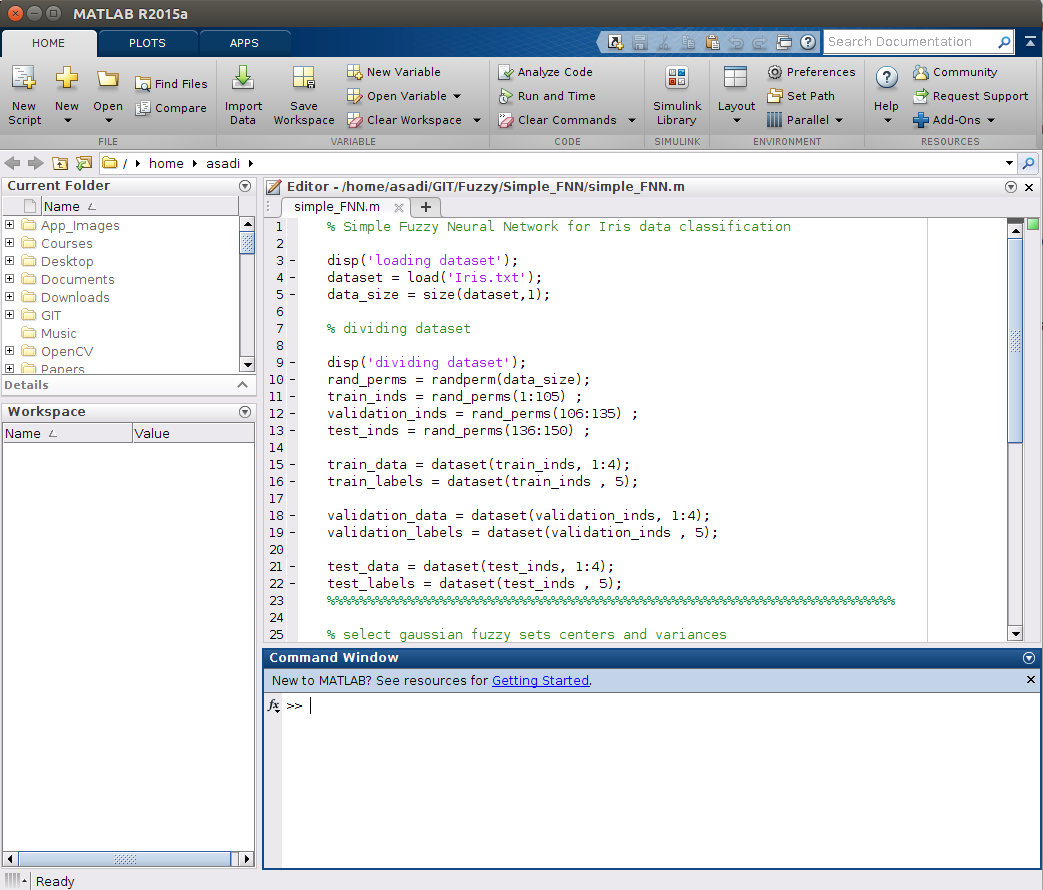
\includegraphics[scale=0.2]{./Imgs/GUI.png}
		\end{figure}
	\end{block}
\end{frame}


\section{Basics}


\begin{frame}{\\ What we will see}
	\begin{itemize}
		\item Getting Started!
			\begin{itemize}
				\item Hello World Again!
				\item Simple Calculations
				\item Hands on Variables
			\end{itemize}
		\item Primitive Data Structures
			\begin{itemize}
				\item Matrices and Vectors
				\item Creating Special Vectors
				\item Functions to create Matrices
			\end{itemize}
		\item Operations
			\begin{itemize}
				\item Matrix Operations
				\item Array Operations
			\end{itemize}
		\item Reading Values of Cells in Matrices and Vectors
	\end{itemize}
\end{frame}


\begin{frame}[fragile]{Getting Started}
	\begin{block}{Hello World Again}
	\begin{itemize}	
		\item Using command window
		\item There is commands for input/output that we will drill into later
		\item A handy one is
			\begin{itemize}
				\item disp(\'this is a message\') $\rightarrow$ prints the message string in command window
			\end{itemize}
		\item The traditional first example!
		\java
			\begin{lstlisting}
				>> disp('Hello World!')
				Hello World!
			\end{lstlisting}
	\end{itemize}	
	
	\end{block}
\end{frame}

\begin{frame}[fragile]{Getting Started}
	\begin{block}{Simple Calculations}
		\begin{itemize}
			\item You can write any desired expression to be calculated and get its results simply in command window.
			\java
				\begin{lstlisting}
					>> 2 + 3
					ans = 
							5
					>> sqrt((pi * 12)^2 / 3 - 57 * cos(pi/3)) 
					ans =
							21.007
				\end{lstlisting}
			\item There exists a complete list of provided functions like $cos()$ and $sqrt()$ available \href{http://mathworks.com/help/matlab/functionlist.html}{here in MATLAB documentation}:\\
			\url{http://mathworks.com/help/matlab/functionlist.html}
		\end{itemize}
	\end{block}
\end{frame}

\begin{frame}[fragile]{Getting Started}
	\begin{block}{Hands on Variables}
		\begin{itemize}
			\item Variables are named places on memory being used in order to keep a value
			\item Each variable has a specific data type
			\item There exists a list of defined data types in MATLAB documents
			\java
				\begin{lstlisting}
					>> a = 2
					a = 
							2
					>> b = 3
					b =
							3
					>> c = a + b
					c =
							5
					>> (c * a * b)^2
					ans =
						900
				\end{lstlisting}
			\item There exists a complete list of provided functions like $cos()$ and $sqrt()$ available \href{http://mathworks.com/help/matlab/functionlist.html}{here}:\\
			\url{http://mathworks.com/help/matlab/functionlist.html}
		\end{itemize}
	\end{block}
\end{frame}

\begin{frame}[fragile]{Primitive data structures}
	\begin{block}{Matrices \& Vectors}
		\begin{itemize}
			\item Almost the most primitive data structures in MATLAB $\rightarrow$ matrices
			\item Defined as bellow:
			\java
				\begin{lstlisting}
	 				>> A = [1 2; 3 4]
	 				A = 		1	2 
	 				     3	4
				\end{lstlisting}
			\item Separate rows by ';' and cols by ',' or ' '
			\item Vectors are special cases of matrices
				\begin{itemize}
					\item [-]\textbf{Row Vector} is an $N*1$ matrix
					\item [-]\textbf{Column Vector} is a $1*M$ matrix
				\end{itemize}
			\item $size(A)$ returns dimensions of matrix $A$
		\end{itemize}
	\end{block}
\end{frame}


\begin{frame}[fragile]{Facilities in Creating Vectors}
	\begin{block}{}
		\begin{itemize}
			\item Creating a vector with equally spaced intervals
			\java
				\begin{lstlisting}
					>> A = 1:0.5:pi
					A =	1.0000	1.5000	2.0000	2.5000	3.0000
				\end{lstlisting}
			\item Creating a vector with $n$ equally spaced intervals
			\java
				\begin{lstlisting}
					>> A = linspace(0, pi, 7)
					A =	0 0.5236	1.0472	1.5708	2.0944	2.6180	3.1416
				\end{lstlisting}
		\end{itemize}
	\end{block}
	\begin{alertblock}{Note}
		\begin{itemize}
			\item [-] MATLAB uses $pi$ to represent $\pi$ and $i$ or $j$ to represent imaginary unit
		\end{itemize}
	\end{alertblock}
\end{frame}



\begin{frame}{Matrices}
	\begin{block}{There is still another useful slide!}
		There exist a list of useful functions being used to create matrices
		\begin{itemize}
			\item[-]$zeros(m,n)$ creates an $m * n$ matrix of all zeros
			\item[-]$ones(m,n)$ creates an $m * n$ matrix of all ones
			\item[-]$eye(m,n)$ creates an $m * n$ identity matrix
			\item[-]$rand(m,n)$ creates an $m * n$ uniformly distributed randoms
			\item[-]$randn(m,n)$ creates an $m * n$ normally distributed randoms
			\item[-]$magic(m)$ creates a square matrix with equal summation of rows, columns and diagonal
			\item[-]$pascal(m)$ creates a square pascal matrix
		\end{itemize}
	\end{block}

\end{frame}

\begin{frame}{Operations}
	\begin{block}{}
		Operations on vectors and matrices are divided into two groups
		\begin{enumerate}
			\item Matrix Operations \\
			Operands of these kind of operations are matrices as whole. 
			\item Array Operations \\
			Operands of these kind of operations are elements of matrices. These kind of operations are being applied to matrices, element by element. 
		\end{enumerate}
	\end{block}
\end{frame}

\begin{frame}{Operations}
	\begin{block}{Matrix Operations}
		\begin{itemize}
			\item [-] $+ \rightarrow $ summation 
			\item [-] $- \rightarrow $ subtraction
			\item [-] $* \rightarrow $ multiplication
			\item [-] $/ \rightarrow $ division  
			\item [-] $\setminus \rightarrow $ left division($ A\setminus B = INV(A) * B$)
			\item [-] $\hat{} \rightarrow $ exponentiation  
		\end{itemize}
	\end{block}
	\begin{block}{Array Operations}
		\begin{itemize}
			\item [-] $.' \rightarrow $ array transpose
			\item [-] $.\hat{} \rightarrow $ array power
			\item [-] $.* \rightarrow $ array multiplication
			\item [-] $./ \rightarrow $ array division  
		\end{itemize}
	\end{block}
\end{frame}

\begin{frame}[fragile]{Reading values of a particle matrix}
	\begin{block}{}
		\begin{itemize}
			\item get value of cell on row 1, col 3 of matrix $A$
			\java
				\begin{lstlisting}
					>> A(1,2)
				\end{lstlisting}
			\item get value of cells on row 2, from col 2 to col 5 of matrix $A$
			\java
				\begin{lstlisting}
					>> A(3,2:5)
				\end{lstlisting}
			\item get value of cells from row 3 to row 6 on col 3 of matrix $A$
			\java
				\begin{lstlisting}
					>> A(3:6,3)
				\end{lstlisting}
			\item get value of cells from row 1 to row 3, from col 2 to row 4 of matrix $A$
			\java
				\begin{lstlisting}
					>> A(1:3,2:4)
				\end{lstlisting}
		\end{itemize}
	\end{block}
\end{frame}

\begin{frame}[fragile]{Reading values of a particle matrix}
	\begin{block}{}
		\begin{itemize}
			\item get value of all cells on row 3 of matrix $A$
			\java
				\begin{lstlisting}
					>> A(3,:)
				\end{lstlisting}
			\item get value of all cells on col 2 of matrix $A$
			\java
				\begin{lstlisting}
					>> A(:,2)
				\end{lstlisting}
			\item get value of all cells of matrix $A$
			\java
				\begin{lstlisting}
					>> A(:,:)
				\end{lstlisting}
		\end{itemize}
	\end{block}
\end{frame}

\section{Exercises}

\begin{frame}{You are what you practice more $_{Richard Carlson}$}
	\begin{block}{}
		\begin{enumerate}
			\item Compute:\\
			$4[2, 32, 42, 55, 2]^T + (-2)[1, 3, 5, 2, -6]^T + [5, -10, 3, 5, 32]^T$
			\item Compute determinant of matrix A without using any function:\\
			\begin{center}
				$A = \begin{bmatrix}
					12 & 3323 & 411\\
					30 & -331 & 345\\
					-12.323 & 34.653 & -34
				\end{bmatrix}$			
			\end{center}
			\item Compute determinant of matrix A using $det()$ function for inner $2*2$ matrices
			\item Do Gauss-Jordan to solve following equations:
			\begin{center}
			$
			\left\{
				\begin{array}{ll}
					x + y + z = 5  \\
					2x + 3y + 5z = 8 \\
					4x + 5z = 2 
				\end{array}
			\right.
			$
			\end{center}
		\end{enumerate}
	\end{block}
\end{frame}
\section{Solving Equations}
\begin{frame}{What we will see}
	\begin{block}{}
		\begin{itemize}
			\item How to  solve a simple equation
			\item How to get more than a response from a function
			\item How to solve a set of equations 
		\end{itemize}
	\end{block}
\end{frame}

\begin{frame}[fragile]{Solve a Simple Equation}
	\begin{block}{}
		\begin{itemize}
			\item Define equations
			\item Define unknowns with \textit{syms}
			\item Use the \textit{'=='} to specify an equation
			\item Use \textit{solve} method to solve the equations
		\end{itemize}
		\java
			\begin{lstlisting}
				>> syms x
				>> eqn = sin(x) == 1;
				>> solx = solve(eqn,x)
				solx =
						pi/2
			\end{lstlisting}
	\end{block}
\end{frame}

\begin{frame}[fragile]{Solve a Simple Equation}
	\begin{block}{}
		\begin{itemize}
			\item There exists some options for \textit{solve} method
			\item A useful one $\rightarrow$ \textit{ReturnConditions}\\
			Returns all solutions under specified conditions
		\end{itemize}
		\java
			\begin{lstlisting}
				>> [solx, params, conds] = solve(eqn, x, 'ReturnConditions', true)
				solx =
				pi/2 + 2*pi*k

				params =
				k

				conds =
				in(k, 'integer')
			\end{lstlisting}
		\begin{alertblock}{Note}
		\begin{itemize}
			\item It is possible to get more than a result from a called function
		\end{itemize}
		\end{alertblock}
	\end{block}
\end{frame}

\begin{frame}[fragile]{Solve a Set of Equations}
	\begin{block}{}
		\begin{itemize}
			\item Use a vector of equations
			\item Use a vector of unknowns
			\item Use \textit{solve()} function to solve all of them
			\java
			\begin{lstlisting}
				>> eqn1 = x + y + z == 6;
				>> eqn2 = x - 2*y + z == 0;
				>> eqn3 = x - z == -2;
				>> [solx, soly, solz]=solve([eqn1, eqn2,eqn3],[x,y,z])
				solx =
				1
				soly =
				2
				solz =
				3
			\end{lstlisting}
		\end{itemize}
	\end{block}
\end{frame}

\begin{frame}[fragile]{Structs}
	\begin{block}{}
		\begin{itemize}
			\item Structs are being used in order to keep a set of different variables packed
			\item Makes working with a set of different variables more convenient
			\item Each struct has a unique name (as same as other variables)
			\item Each variable inside a struct has a unique name
			\item Value of each inner variables in a struct can be read using '.'
		\end{itemize}
	\end{block}
	\begin{block}{In the example on next page...}
		\begin{itemize}
			\item \textit{S} is the name of a struct holding all parameters returned by \textit{solve} function
			\item The name of inner variables in \textit{S} is the same as their name when returned by \textit{solve} function
			\item The value of each inner variable is accessible using '.'
		\end{itemize}
	\end{block}
\end{frame}

\begin{frame}[fragile]{Structs}
	\begin{block}{}
			\java
				\begin{lstlisting}
				>> S = solve([eqn1, eqn2],[x,y,z],'ReturnConditions' , true)
					S = 
						x: [1x1 sym]
						y: [1x1 sym]
						z: [1x1 sym]
						parameters: [1x1 sym]
						conditions: [1x1 sym]
				>> S.x
					ans =
						4 - z1
				>> S.z
					ans =
						z1
				>> S.parameters
					ans =
						z1
 				\end{lstlisting}
	\end{block}
\end{frame}

\section{Figures and Plots}

\begin{frame}{What we will see}
	\begin{block}{}
		\begin{itemize}
			\item How to create  a new figure
			\item How to use plot for drawing 2D curves
			\item How to use scatter for drawing 2D points 
		\end{itemize}
	\end{block}
\end{frame}


\begin{frame}{Figures}
	\begin{block}{}
		\begin{itemize}
			\item The instruction \textit{'figure'}, creates an empty window
			\item The created window will be used by plots
			\item Each single call on \textit{'figure'} will generate a new window
			\item It does not take any parameter
		\end{itemize}
	\end{block}
	\begin{alertblock}{Note that...}
		\begin{itemize}
			\item The first figure will be created automatically and does not need to any figure call, but the others should have a figure call in essential cases.
		\end{itemize}
	\end{alertblock}
\end{frame}

\begin{frame}[fragile]{Plot Function}
	\begin{block}{}
		\begin{itemize}
			\item Plots a line over input points
			\item For each point the specific $(x,y)$ pair is required
			\item A separated vector for all $x_s$ and $y_s$ is required
			\vspace{10pt}
			\begin{tabular}{p{0.4\textwidth}p{0.4\textwidth}}
			\begin{minipage}{0.4\textwidth}
			\java
				\begin{lstlisting}
					>> X = -2:0.0001:2;
					>> Y = X.^2 + 1;
					>> plot(X,Y)
				\end{lstlisting}
			
			\end{minipage}
			&
			\begin{minipage}{0.4\textwidth}
			\begin{figure}[H]
				\centering
				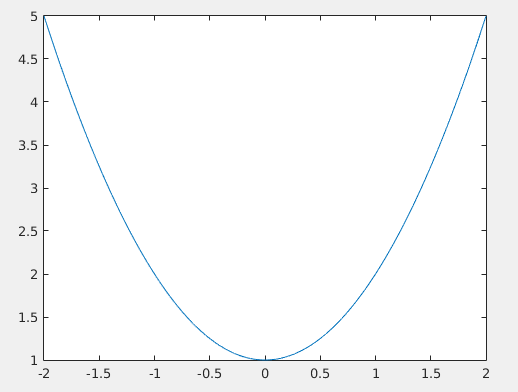
\includegraphics[scale=0.25]{./Imgs/plot1.png}
			\end{figure}
			
			\end{minipage}
			\end{tabular}
		\end{itemize}
	\end{block}
\end{frame}

\begin{frame}[fragile]{Plot Function}
	\begin{block}{Some options...}
		\begin{itemize}
			\item use \textit{'hold on'} to plot more than one curve
			\vspace{10pt}
			\begin{tabular}{p{0.4\textwidth}p{0.4\textwidth}}
			\begin{minipage}{0.4\textwidth}
			\java
				\begin{lstlisting}
>> X = -2:0.0001:2;
>> Y = X.^2 + 1;
>> Z = sqrt(abs(5*X));
>> plot(X,Y)
>> hold on;
>> plot(X,Z)
				\end{lstlisting}
			
			\end{minipage}
			&
			\begin{minipage}{0.4\textwidth}
			\begin{figure}[H]
				\centering
				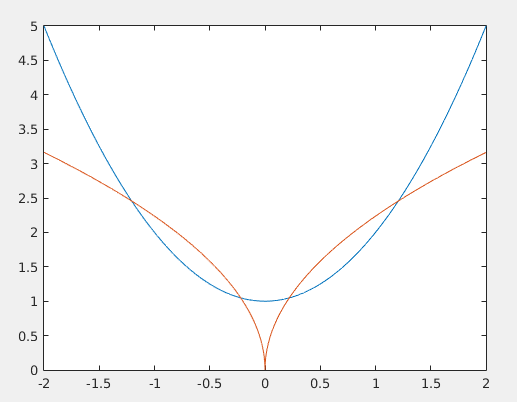
\includegraphics[scale=0.25]{./Imgs/plot2.png}
			\end{figure}
			
			\end{minipage}
			\end{tabular}
		\end{itemize}
	\end{block}
\end{frame}



\begin{frame}[fragile]{Scatter Function}
	\begin{block}{}
		\begin{itemize}
			\item \textit{Scatter}, draws points given their coordination
			\begin{tabular}{p{0.4\textwidth}p{0.4\textwidth}}
			\begin{minipage}{0.4\textwidth}
			\java
				\begin{lstlisting}
>> X = 1:10;
>> Y = -X;
>> scatter(X,Y)
				\end{lstlisting}
			
			\end{minipage}
			&
			\begin{minipage}{0.4\textwidth}
			\begin{figure}[H]
				\centering
				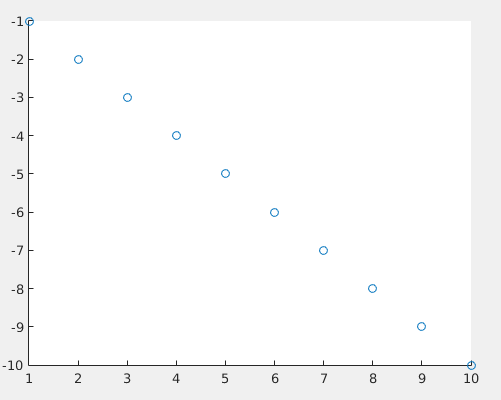
\includegraphics[scale=0.2]{./Imgs/scatter1.png}
			\end{figure}
			
			\end{minipage}
			\end{tabular}
			
			\item The area of each point can be specified by third parameter
			
			\begin{tabular}{p{0.4\textwidth}p{0.4\textwidth}}
			\begin{minipage}{0.4\textwidth}
			\java
				\begin{lstlisting}
>> X = 1:10;
>> Y = -X;
>> A = 10*X;
>> scatter(X,Y,A)
				\end{lstlisting}
			
			\end{minipage}
			&
			\begin{minipage}{0.4\textwidth}
			\begin{figure}[H]
				\centering
				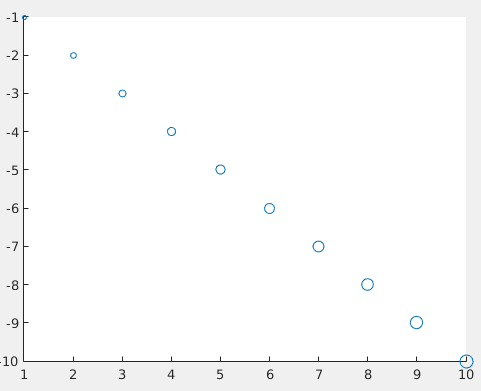
\includegraphics[scale=0.2]{./Imgs/scatter2.png}
			\end{figure}
			
			\end{minipage}
			\end{tabular}
			
			
		\end{itemize}
	\end{block}
\end{frame}


\section{Exercises}

\begin{frame}{}
	\begin{block}{An ounce of practice is generally worth more than a ton of theory$_{Ernst F. Schumacher}$}
		\begin{enumerate}
			\item Plot each of following curves in a 3d space (use \textit{plot3}  and \textit{scatter3})
			\item Solve the set of equations two by two and find solution points
			\item Specify solution points on the plot
			\begin{center}
			$
			\left\{
				\begin{array}{ll}
					sin(x) + cos(y) + z = 3  \\
					2x + 3sin(y) + 5z = 2\pi + 5 \\
					4x + 5z = 4\pi + 5 
				\end{array}
			\right.
			$
			\end{center}
		\end{enumerate}
	\end{block}
\end{frame}


\section{Programming in MATLAB}

\begin{frame}{What we will see}
	\begin{block}{}
		\begin{itemize}
			\item Conditional statements
			\item For Loops
			\item While Loops
		\end{itemize}
	\end{block}
\end{frame}


\begin{frame}[fragile]{Conditional Statements}
	\begin{block}{}
		\begin{itemize}
			\item Control the conditions under which some operations needed to be accomplished
			\item There exist several shapes of statements which are referred to as \textit{'IF' Statements}
			\item Use \textit{(if-end)} form for statements that are required to be accomplished just in true cases of a certain statement
			\item Use \textit{(if-else-end)} form for deciding on executing one of two specified statements according to value of the one existing condition
			\item Use \textit{(if-elseif-end)} form for deciding on executing one of more than two specified statements according to value of the condition corresponding to each statement
			\item The examples on next pages will through light on the fact.
		\end{itemize}
	\end{block}
\end{frame}

\begin{frame}[fragile]{IF-END}
	\begin{block}{}
				\java
				\begin{lstlisting}
				>>	x = 3;
				if(x == 2)
						disp('statement 1');
				end				
				>>	x = 2;
				if(x == 2)
						disp('statement 2');
				end
				statement 2
				\end{lstlisting}
	\end{block}

	\begin{block}{Notes on the example...}
		\begin{itemize}
			\item In the above example, the statement inside the first \textit{if} clause won't be executed because there $x \neq 2$. 
			\item On the other hand, in the second \textit{if} clause, as $x == 2$ is true, the inside statement will be executed and \textit{\'statement 2\'} will be printed on console.
		\end{itemize}
	\end{block}

\end{frame}

\begin{frame}[fragile]{IF-ELSE-END}
	\begin{block}{}
				\java
				\begin{lstlisting}
				>>	x = 3;
				if(x == 2)
						disp('The X is equal to 2');
				else
						disp('NOP! X is not equal to 2');
				end
				
				NOP! X is not equal to 2

				>>	x = 2;
				if(x == 2)
						disp('The X is equal to 2');
				else
						disp('NOP! X is not equal to 2');
				end
				
				The X is equal to 2
				\end{lstlisting}
	\end{block}

\end{frame}

\begin{frame}{IF-ELSE-END}
	\begin{block}{Notes on the example...}
		\begin{itemize}
			\item In the above example at first attempt, the statement inside the \textit{if} clause won't be executed because $x \neq 2$, therefore, the inner statement of \textit{else} clause will be executed.
			\item At the second attempt, $x == 2$ so the inner statement of \textit{if} clause will be executed and the left won't be launched.
		\end{itemize}
	\end{block}
\end{frame}	
	

\begin{frame}[fragile]{IF-ELSEIF-END}
	\begin{block}{}
				\java
				\begin{lstlisting}
				>>	x = 3;
				if(x == 1)
						disp('The X is equal to 1');
				elseif (x == 2)
						disp('The X is equal to 2');
				elseif (x == 3)
						disp('The X is equal to 3');
				elseif (x == 4)
						disp('The X is equal to 4');
				else
						disp('NOP! X is not equal to 1, 2, 3 or 4');
				end
				
				The X is equal to 3
				\end{lstlisting}
	\end{block}

\end{frame}

\begin{frame}{IF-ELSEIF-END}
	\begin{block}{Notes on the example...}
		\begin{itemize}
			\item In the above example at first attempt, the statement inside the \textit{if} clause won't be executed because $x \neq 1$, therefore, the condition on first \textit{elseif} clause will be checked. As $x \neq 2$, the inner statement of first \textit{elseif} clause would be ignored and the condition of the next \textit{elseif} clause would be checked. 
			\item If no conditions satisfies, the inner statement of \textit{else} clause would be executed.
			\item The number of \textit{elseif} clauses is unlimited.
			\item The existence of \textit{else} clause is optional, but at most one \textit{else} clause is allowd.
			\item At the second attempt, $x == 2$ so the inner statement of \textit{if} clause will be executed and the left won't be launched.
		\end{itemize}
	\end{block}
\end{frame}	
	
	
		
\begin{frame}[fragile]{FOR Loops}
	\begin{block}{}
		\begin{itemize}
			\item Repeat a set of statements a specific number of times
			\item The general syntax
			\java
				\begin{lstlisting}
					>> 
						for <counter variable> = <range of values>
							<the set of statements need to repeat>
						end
				\end{lstlisting}
			\item \textit{counter variable} proceeds in \textit{range of values} along with repeating the \textit{specified statements}.
		\end{itemize}	
	\end{block}
\end{frame}

\begin{frame}[fragile]{FOR Loops}
	\begin{block}{}
				\java
				\begin{lstlisting}
					>> 
						for x = 1:5
							disp('this is the value of x>>');
							disp(x);
						end

this is the value of x>>
     1
this is the value of x>>
     2
this is the value of x>>
     3
this is the value of x>>
     4
this is the value of x>>
     5

				\end{lstlisting}

	\end{block}
\end{frame}
	
	
\begin{frame}[fragile]{WHILE Loops}
	\begin{block}{}
		\begin{itemize}
			\item Repeat a set of statements while a specific condition is true
			\item The general syntax
			\java
				\begin{lstlisting}
					>> 
						while (<condition>)
							<the set of statements need to repeat>
						end
				\end{lstlisting}
			\item The specified condition will be checked, if is true, then all of specified statements inside the \textit{while} will be executed. After each round of execution, the condition will be checked again and the statements will be executed if condition is true. As the condition turns to false, the execution will be stopped and control flow will chase the statements after while.
			\item The example on next page is an equivalent of the previous example!
		\end{itemize}	
	
	\end{block}
\end{frame}
	

\begin{frame}[fragile]{WHILE Loops}
	\begin{block}{}
		\java
		\begin{lstlisting}
		>>
		 x = 0;
		 while(x < 5)
		 x = x + 1;
		 disp('This is the value of x>>');
		 disp(x);
		 end
		 
This is the value of x>>
     1
This is the value of x>>
     2
This is the value of x>>
     3
This is the value of x>>
     4
This is the value of x>>
     5

		\end{lstlisting}
	\end{block}

\end{frame}	
	
\section{Exercises}
\begin{frame}[fragile]{}
	\begin{block}{Practice puts brain in your muscles.$_{Sam Snead}$}
		\begin{enumerate}
\item 
Given the vector x = [1 8 3 9 0 1], create a short set of commands that will
\\
   a. Add up the values of the elements (Check with sum.) 
   \\
   b. Computes the running sum (for element j, the running sum is the sum of the
      elements from 1 to j, inclusive.  Check with cumsum.)
      \\
   c. computes the sine of the given x-values (should be a vector)          
   
\item 
Compute the value of pi using the following series

\begin{center}
$
\frac{\pi ^ 2 - 8}{16} = \Sigma_{n=1}^\infty \frac{1}{(2n-1)^2(2n+1)^2}
$
\end{center}


   How many terms are needed to obtain an accuracy of 1e-12?  How accurate is 
   the sum of 100 terms of this series?

    		\end{enumerate}
	\end{block}
\end{frame}
	
\end{document}

